\documentclass[border=4pt]{standalone}
\usepackage[T1]{fontenc}
\usepackage{helvet}
\renewcommand{\familydefault}{\sfdefault}
\usepackage{graphicx}
\usepackage{caption}
\usepackage{amsmath}
\captionsetup{font={sf,footnotesize},labelfont={sf,bf,footnotesize},justification=justified,singlelinecheck=false}
\begin{document}
\setcounter{figure}{0}
\begin{minipage}{7.20in}
\centering
\begin{figure}[htbp]
    \centering
    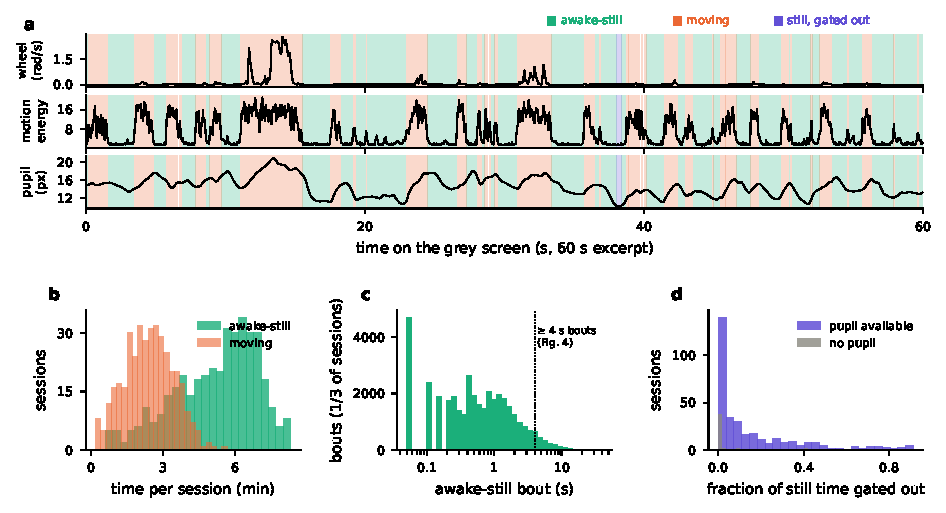
\includegraphics[width=\linewidth]{fig1_states_panels.pdf}
    \caption{Defining awake stillness on the passive grey screen. \textbf{a} Example grey-screen minute (session 5d6aa933): wheel speed, left-camera motion energy and pupil diameter, with awake-still (green), moving (orange) and still-but-gated-out (violet) 50\,ms bins. \textbf{b} Awake-still and moving time per session (389 sessions). \textbf{c} Durations of awake-still bouts (log axis); true-offset bouts of at least 4\,s enter the within-bout analyses. \textbf{d} Fraction of still time removed by the anti-sleep gate (pupil below the 10th percentile of the task-period pupil, or more than 30\,s since the last movement).}
    \label{fig:states}
\end{figure}
\end{minipage}
\end{document}
